\section{Sector-NN calibration: corpus partition and per-sector breakdown}\label{sec:supp_sector_nn}

We decomposed the headline three-way RMSE comparison along two axes and observed that the ETF and Technology sectors together carried roughly three-quarters of the corpus, the sector NN reduced RMSE in every sector over the shared NN with the largest gains in ETF and financials, and the per-ticker residual error concentrated on a small set of technology and healthcare names (Tables~\ref{tab:sector_map}, \ref{tab:per_sector}, \ref{tab:worst_tickers}). The corpus partition that defined the sector grouping is reported in Table~\ref{tab:sector_map}, the per-sector RMSE decomposition in Table~\ref{tab:per_sector}, and the per-ticker fit ranking under the sector NN in Table~\ref{tab:worst_tickers}.

\begin{table}[ht]
\centering
\caption{Sector partition of the 31-ticker ladder. Each ticker appeared on at least one of fifteen capture dates (2026-04-14 through 2026-05-11); per-sector observation counts were pooled across dates. ETF observation counts were substantially larger than other sectors because SPY, QQQ, and IWM carried far deeper strike ladders than individual-name chains.}\label{tab:sector_map}
\resizebox{\textwidth}{!}{%
\begin{tabular}{lrl}
\toprule
Sector & Observations & Tickers \\
\midrule
ETF        & 102{,}738 & IWM, QQQ, SPY \\
Technology &  68{,}334 & AAPL, AMD, AVGO, GOOG, INTC, META, MSFT, MU, NVDA, QCOM \\
Healthcare &  26{,}387 & ABBV, AMGN, BMY, JNJ, LLY, MRNA, PFE, UNH \\
Financials &  17{,}938 & BAC, GS, JPM, WFC \\
Retail     &  11{,}320 & TGT, UPS, WMT \\
Energy     &   7{,}832 & CVX, OXY, XOM \\
\bottomrule
\end{tabular}}
\end{table}

\begin{table}[ht]
\centering
\caption{Per-sector RMSE (\% IV) across the three calibration strategies on the 31-ticker ladder. The sector NN reduced RMSE in every sector over the shared NN, with the largest absolute gains in ETF and financials, where the global shape poorly represented the local geometry. Healthcare and technology retained the largest residual errors, reflecting within-sector smile heterogeneity that a single shared sector $\psi$ could not absorb.}\label{tab:per_sector}
\begin{tabular}{lrrrr}
\toprule
Sector & Parametric & Shared NN & Sector NN & Obs.\ count \\
\midrule
ETF        & 10.54 &  8.69 &  6.10 & 102{,}738 \\
Financials &  9.05 &  7.79 &  6.70 &  17{,}938 \\
Energy     &  9.36 &  8.24 &  7.88 &   7{,}832 \\
Retail     & 11.73 & 10.23 &  9.50 &  11{,}320 \\
Healthcare & 13.49 & 12.71 & 12.53 &  26{,}387 \\
Technology & 15.58 & 15.31 & 14.47 &  68{,}334 \\
\bottomrule
\end{tabular}
\end{table}

\begin{table}[ht]
\centering
\caption{Best and worst individual ticker fits under the sector-specific NN calibration, ranked by RMSE across all 31 tickers. The best fits were dominated by the broad-market ETFs and the deep-liquidity financials (GS, JPM); the worst fits were concentrated in technology (QCOM, MU, INTC, AMD) and healthcare (PFE, MRNA), where within-sector smile heterogeneity was largest. PFE and BMY remained the only tickers below the 2{,}000-observation per-ticker threshold.}\label{tab:worst_tickers}
\begin{tabular}{llrrl}
\toprule
Rank & Ticker & Obs.\ count & RMSE (\% IV) & Sector \\
\midrule
\multicolumn{5}{l}{\emph{Best 5}} \\
 1 & GS   &  8{,}772 & 5.40 & Financials \\
 2 & SPY  & 42{,}224 & 6.02 & ETF \\
 3 & IWM  & 21{,}368 & 6.11 & ETF \\
 4 & QQQ  & 39{,}146 & 6.17 & ETF \\
 5 & JPM  &  3{,}720 & 6.18 & Financials \\
\midrule
\multicolumn{5}{l}{\emph{Worst 5}} \\
27 & PFE  &  1{,}300 & 17.66 & Healthcare \\
28 & AMD  &  4{,}566 & 17.74 & Technology \\
29 & INTC &  3{,}417 & 17.78 & Technology \\
30 & MU   &  6{,}619 & 18.45 & Technology \\
31 & QCOM &  3{,}375 & 21.46 & Technology \\
\bottomrule
\end{tabular}
\end{table}

\subsection{Leave-one-date-out validation on the fifteen-date corpus}\label{sec:supp_loo}

We held out the latest capture (2026-05-11) and retrained the sector $\psi_{\text{NN}}$ on the remaining fourteen dates as a leave-one-date-out check, and observed that the held-out test RMSE landed within $0.68\%$ IV of the pooled train RMSE (Table~\ref{tab:loo_sector_nn}). The held-out day comprised 14{,}442 observations ($6.2\%$ of the corpus); we trained the six sector networks on the remaining fourteen dates using identical architecture, schedule, and seed, standardised only on the training rows so the test split could not leak through the input scaling, and evaluated test RMSE on the held-out day. The overall train RMSE of $10.21\%$ matched the full-corpus in-sample number of $10.24\%$ within rounding, confirming that withholding one day did not perturb the fit, and the held-out test RMSE of $10.89\%$ left a generalization gap of only $+0.68\%$ IV pooled across all six sectors. The gap was strongly sector-specific: four of six sectors (ETF, Financials, Healthcare, Tech) carried negative or small-positive gaps, while Energy ($+2.23\%$) and Retail ($+3.96\%$) showed larger positive gaps consistent with the small per-sector sample sizes on the holdout day amplifying single-name idiosyncrasies. The overall pattern was consistent with the temporal-holdout result of §\ref{sec:earnings_holdout}: with no earnings prints inside the holdout, the sector NN generalized to an unseen capture date with $\sim 7\%$ relative degradation in RMSE, far below what an overfit model would exhibit.

\begin{table}[ht]
\centering
\caption{Leave-one-date-out validation of the sector NN, holding out 2026-05-11. Per-sector train and test RMSE (\% IV) and gap (test $-$ train). The pooled gap of $+0.68\%$ IV is small relative to the in-sample RMSE itself, indicating that the architecture does not overfit the fifteen-date corpus.}\label{tab:loo_sector_nn}
\begin{tabular}{lrrr}
\toprule
Sector & Train (\%) & Test (\%) & Gap (\%) \\
\midrule
ETF        &  6.12 &  5.87 & $-0.25$ \\
Financials &  6.72 &  6.32 & $-0.40$ \\
Healthcare & 12.58 & 12.00 & $-0.58$ \\
Tech       & 14.45 & 15.04 & $+0.58$ \\
Energy     &  7.74 &  9.97 & $+2.23$ \\
Retail     &  9.21 & 13.17 & $+3.96$ \\
\midrule
Pooled     & 10.21 & 10.89 & $+0.68$ \\
\bottomrule
\end{tabular}
\end{table}

\subsection{Walk-forward temporal validation across the fifteen-date corpus}\label{sec:supp_walk_forward}

We extended the leave-one-date-out check to a full walk-forward sweep across the fifteen-date corpus: for $k = 5,\ldots,14$, we trained the sector $\psi_{\text{NN}}$ on the first $k$ sorted ladder dates (Configuration-A pooled control, 2-input $\psi$) and tested on date $k+1$, producing ten folds (Table~\ref{tab:walk_forward}). The fold-wise pattern was the same one isolated by the earnings-holdout study: median test RMSE was $11.08\%$ IV and median generalization gap was $+2.02\%$, but the distribution was driven by a small number of earnings-blowup folds rather than uniform temporal degradation. The largest single-fold gap was $+9.41\%$ on the $k = 6$ fold (test day 2026-04-23), the same INTC print day that drove the headline Configuration-A gap of $+4.99\%$ in Table~\ref{tab:earnings_holdout}; that fold tested on 04-23 alone, while Configuration-A averaged 04-23 with the calmer 04-24, which is why the standalone fold gap was roughly twice as large. The non-earnings $k = 14$ fold (test day 2026-05-11, no earnings prints in the window) produced a gap of $+0.68\%$, reproducing the leave-one-date-out result of Table~\ref{tab:loo_sector_nn} and confirming that the multi-date pool generalizes faithfully when no scheduled event sits inside the test window.

\begin{table}[ht]
\centering
\caption{Walk-forward temporal validation across the fifteen-date corpus. For each $k$, the sector $\psi_{\text{NN}}$ was trained on the first $k$ sorted ladder dates and tested on date $k+1$; standardization was computed from the training rows only. The earnings column flags folds in which any test-day row sat within $\pm 3$ days of an earnings print for the ticker or any same-sector peer. The $k = 6$ fold (test 2026-04-23) reproduces the INTC-print blowup that drives the Configuration-A gap in Table~\ref{tab:earnings_holdout}; the non-event $k = 14$ fold reproduces the leave-one-date-out result of Table~\ref{tab:loo_sector_nn}.}\label{tab:walk_forward}
\begin{tabular}{rlrrrrl}
\toprule
$k$ & Test date & $N_{\text{tr}}$ & $N_{\text{te}}$ & Train (\%) & Test (\%) & Gap (\%) \\
\midrule
 5 & 2026-04-22 &  88{,}346 & 15{,}551 &  7.61 & 10.47 & $+2.87$ \\
 6 & 2026-04-23 & 103{,}897 & 11{,}482 &  8.05 & 17.45 & $+9.41$ \\
 7 & 2026-04-24 & 115{,}379 & 15{,}351 &  9.34 &  7.79 & $-1.55$ \\
 8 & 2026-04-27 & 130{,}730 & 11{,}379 &  9.16 & 12.57 & $+3.41$ \\
 9 & 2026-04-28 & 142{,}109 & 16{,}776 &  9.42 & 12.86 & $+3.44$ \\
10 & 2026-04-29 & 158{,}885 & 16{,}811 &  9.78 & 13.12 & $+3.34$ \\
11 & 2026-05-01 & 175{,}696 & 14{,}825 & 10.11 & 10.08 & $-0.03$ \\
12 & 2026-05-06 & 190{,}521 & 17{,}293 & 10.10 & 11.28 & $+1.18$ \\
13 & 2026-05-08 & 207{,}814 & 12{,}293 & 10.18 & 10.82 & $+0.64$ \\
14 & 2026-05-11 & 220{,}107 & 14{,}442 & 10.21 & 10.89 & $+0.68$ \\
\midrule
\multicolumn{4}{l}{Median across 10 folds}    & --- & 11.08 & $+2.02$ \\
\multicolumn{4}{l}{Mean   across 10 folds}    & --- & 11.73 & $+2.34$ \\
\bottomrule
\end{tabular}
\end{table}

\subsection{Static-arbitrage diagnostic on the calibrated $\psi$ surfaces}\label{sec:supp_static_arb}

We tested the calibrated $\psi$ surfaces against the standard no-arbitrage conditions $\partial^2 C/\partial K^2 \geq 0$ (butterfly) and $\partial C/\partial T \geq 0$ (calendar) on a $20\times 20$ moneyness--maturity grid ($K/S \in [0.80, 1.20]$ log-spaced, DTE $\in [7, 365]$ log-spaced), pricing European calls through the same 200-step CRR pricer used elsewhere in the calibration and evaluating central second differences in $K$ and forward first differences in $T$ on each grid. Across the six sector surfaces (one representative ticker per sector, with $\theta_i$ taken from that ticker) and the two per-ticker surfaces used in §\ref{sec:scenarios} (GS and LLY), butterfly violations averaged 9.76\% of grid points and calendar violations averaged 0.76\% (Table~\ref{tab:static_arb}). Calendar violations were essentially absent on every surface, consistent with the monotone term-structure shape the network learned; butterfly violations clustered in the deep moneyness wings ($K/S \lesssim 0.85$ and $K/S \gtrsim 1.15$) where the corpus carried fewer observations and the network had to extrapolate the curvature. The unconstrained neural surrogate has no structural guarantee of butterfly convexity, and we did not impose a no-arbitrage penalty during training; we report the violation rates here as a known limitation rather than a corrected feature, with no-arbitrage-aware extensions reserved for future work.

\begin{table}[ht]
\centering
\caption{Static no-arbitrage diagnostic on eight calibrated $\psi$ surfaces, evaluated on a $20\times 20$ moneyness--maturity grid via 200-step CRR European call prices. Butterfly violations are grid points where $\partial^2 C/\partial K^2 < 0$ (computed by central second difference on the 18 inner strikes per row, 360 cells per surface); calendar violations are grid points where $\partial C/\partial T < 0$ (forward first difference, 380 cells per surface).}\label{tab:static_arb}
\begin{tabular}{lrrrr}
\toprule
Surface             & Butterfly viol. & Frac.\ (\%) & Calendar viol. & Frac.\ (\%) \\
\midrule
ETF / SPY (sector)        &  56 / 360 & 15.56 & 23 / 380 & 6.05 \\
Tech / NVDA (sector)      &  17 / 360 & 4.72 & 0 / 380 & 0.00 \\
Healthcare / LLY (sector) &  20 / 360 & 5.56 & 0 / 380 & 0.00 \\
Financials / GS (sector)  &  54 / 360 & 15.00 & 0 / 380 & 0.00 \\
Retail / WMT (sector)     &  45 / 360 & 12.50 & 0 / 380 & 0.00 \\
Energy / XOM (sector)     &  24 / 360 & 6.67 & 0 / 380 & 0.00 \\
GS per-ticker             &  36 / 360 & 10.00 & 0 / 380 & 0.00 \\
LLY per-ticker            &  29 / 360 & 8.06 & 0 / 380 & 0.00 \\
\midrule
Aggregate                 & 281 / 2{,}880 & 9.76 & 23 / 3{,}040 & 0.76 \\
\bottomrule
\end{tabular}
\end{table}

\section{Holdout diagnostics motivating the earnings-aware mechanism}\label{sec:supp_earnings_diag}

We decomposed the holdout test error on the Tech sector across the pooled control (A) and the earnings-aware fit (C) and traced the Configuration-C improvement to the peer-coupling feature: tickers whose own prints fell outside the holdout but whose sector peers printed during it received the largest test-RMSE reductions, while INTC, the print-day ticker, was the one Tech name to worsen (Table~\ref{tab:tech_pivot}). The decomposition rested on two preceding diagnostics that established the holdout RMSE jump as a localized earnings response rather than a broad-market regime shift. First, the broad-market volatility index VIX traced a flat path through the holdout window: VIX closed at comparable levels on the final training day and the two holdout days, with no intraday excursion during the holdout that approached even a one-standard-deviation move relative to the trailing six-day window. A regime-shift hypothesis required the index to move materially over the holdout, and it did not. Second, the per-ticker ATM~IV trace revealed that the IV expansion on 04-23 and 04-24 was concentrated entirely in the technology sector, and within that sector concentrated on the names with earnings prints inside or adjacent to the holdout window: INTC (which printed inside the window), MSFT, META, and GOOG all exhibited ATM~IV elevations of 5 to 30 percentage points relative to their training-block baselines, while non-Tech names traced ATM~IV paths consistent with their pre-holdout levels. The combination established that the holdout RMSE jump was not a market-wide effect that the architecture had failed to absorb but a localized response to the earnings calendar, and it directly motivated the earnings indicator and peer-coupling feature reported in Configuration~C of Table~\ref{tab:earnings_holdout}. INTC, the print-day ticker, was the one Tech name to worsen under the earnings-aware fit because its $+2192\%$ EPS surprise produced a post-print IV crush that no calendar-based indicator could anticipate.

\begin{table}[ht]
\centering
\caption{Per-ticker test RMSE on the Tech sector across the pooled control (A) and the earnings-aware fit (C). Columns $e$ and $e^{\text{peer}}$ report the median signed days-to-earnings and the minimum same-sector peer distance for each ticker on the holdout days. The largest gains accrued to tickers whose peers printed within the holdout (QCOM, AMD, META, MSFT, GOOG); INTC, the print-day ticker, was the one name that worsened, reflecting an unanticipated outcome that no calendar-based indicator could absorb.}\label{tab:tech_pivot}
\begin{tabular}{lrrrrr}
\toprule
Ticker & $e$ & $e^{\text{peer}}$ & A: pooled (\%) & C: earnings-aware (\%) & $\Delta$ (\%) \\
\midrule
QCOM & $+5$  & $1$ & 41.66 & 37.59 & $-4.07$ \\
AMD  & $+11$ & $1$ & 40.07 & 36.50 & $-3.57$ \\
META & $+5$  & $1$ & 14.32 & 10.73 & $-3.59$ \\
MSFT & $+5$  & $1$ & 14.00 & 10.73 & $-3.28$ \\
GOOG & $+5$  & $1$ &  9.87 &  7.90 & $-1.97$ \\
MU   & $-30$ & $1$ & 16.95 & 15.59 & $-1.36$ \\
AAPL & $+6$  & $1$ & 10.42 & 10.34 & $-0.08$ \\
AVGO & $+30$ & $1$ & 12.58 & 12.83 & $+0.24$ \\
NVDA & $+26$ & $1$ &  9.43 & 10.47 & $+1.05$ \\
INTC & $-1$  & $5$ & 33.17 & 35.94 & $+2.77$ \\
\bottomrule
\end{tabular}
\end{table}

\section{Short-premium scenarios: P\&L statistics and cross-ticker validation}\label{sec:supp_short_premium}

We tabulated the moments and tail statistics per contract for the GS 31-day forward simulation and observed the short-premium asymmetry that the main-text figures rendered qualitatively: a thin-tailed right side with a hard ceiling at the entry premium, paired with a long left tail that extended an order of magnitude beyond the median (Table~\ref{tab:gs_scenario}). The model's $t=0$ Leisen-Reimer fair value sat essentially at the market mid on both contracts (entry edge $+\$0.75$ on the put, $-\$0.02$ on the call), confirming the per-ticker $\psi_{\mathrm{NN}}$ matched the 04-28 GS market IV. The dispersion was larger on the call leg (std $\$51.58$ vs.\ $\$34.12$), and the worst-case loss on the call ($-\$484.57$) exceeded the worst put loss ($-\$323.42$) by a factor of $1.50$, despite the call collecting a smaller entry premium.

\begin{table}[ht]
\centering
\caption{Terminal P\&L statistics from 1{,}000 GS 31-day forward simulations of the real 2026-05-29 \$890 put and \$970 call. Entry premium was the market mid from the 2026-04-28 capture (GS spot $S_0 = \$926.38$). The model's $t=0$ Leisen-Reimer fair value at NN-IV was reported as a reference; statistics are per contract.}
\label{tab:gs_scenario}
\begin{tabular}{lrr}
\toprule
Statistic & Short put (\$) & Short call (\$) \\
\midrule
Strike $K$                  & 890        & 970       \\
Market mid (entry premium)  & $+16.51$   & $+16.09$  \\
Model $t=0$ fair value      & $+17.26$   & $+16.07$  \\
Entry edge (model $-$ market) & $+0.75$  & $-0.02$   \\
\midrule
Mean P\&L                    &  $+1.52$  &  $-9.00$  \\
Median P\&L                  & $+16.51$  & $+16.09$  \\
Std P\&L                     &  $34.12$  &  $51.58$  \\
5\%-tile P\&L                & $-76.13$  & $-113.16$ \\
Worst-case P\&L              & $-323.42$ & $-484.57$ \\
Premium kept in full         & $72.2\%$  & $64.3\%$  \\
\bottomrule
\end{tabular}
\end{table}

\begin{algorithm}[ht]
\caption{Path-conditional Greeks via central finite differences on the LR pricer}\label{alg:greeks}
\begin{algorithmic}[1]
\Require State $(S, \sigma, \tau)$ with $\tau = T - t$; contract $(K, r)$; LR depth $N_{\mathrm{LR}}$; spot bump $h_S$ (relative); IV bump $h_\sigma$ (absolute).
\Ensure $\Delta$, $\Gamma$, Vega.
\State $P_+^S \gets \mathrm{LR}_{N_{\mathrm{LR}}}(S(1+h_S),\, K,\, \sigma,\, \tau,\, r)$
\State $P_-^S \gets \mathrm{LR}_{N_{\mathrm{LR}}}(S(1-h_S),\, K,\, \sigma,\, \tau,\, r)$
\State $P_0  \gets \mathrm{LR}_{N_{\mathrm{LR}}}(S,\, K,\, \sigma,\, \tau,\, r)$
\State $P_+^\sigma \gets \mathrm{LR}_{N_{\mathrm{LR}}}(S,\, K,\, \sigma + h_\sigma,\, \tau,\, r)$
\State $P_-^\sigma \gets \mathrm{LR}_{N_{\mathrm{LR}}}(S,\, K,\, \sigma - h_\sigma,\, \tau,\, r)$
\State $\Delta \gets \dfrac{P_+^S - P_-^S}{2\, h_S\, S}$
\State $\Gamma \gets \dfrac{P_+^S - 2\, P_0 + P_-^S}{(h_S\, S)^2}$
\State $\mathrm{Vega} \gets \dfrac{P_+^\sigma - P_-^\sigma}{2\, h_\sigma}$ \Comment{per unit IV; multiply by $0.01$ for per-$1\%$ IV}
\State \Return $(\Delta,\, \Gamma,\, \mathrm{Vega})$
\end{algorithmic}
\end{algorithm}

\begin{figure}[ht]
\centering

\includegraphics[width=\textwidth]{sections/figures/gs/gs_short_greeks.pdf}
\caption{Leisen-Reimer American Greeks ($\Delta$, $\Gamma$, Vega) at the GS put and call strikes over the 31-day horizon, computed by central finite differences (Algorithm~\ref{alg:greeks}) on the 201-step Leisen-Reimer pricer at the per-path NN-IV ($h_S = 1.5\% S_t$ for $\Delta$/$\Gamma$, $d\sigma = \pm 0.005$ for Vega). Long-Greek convention: short-position Greeks are the negatives. Top row: $\Delta$. Middle: $\Gamma$, exhibiting the short-gamma spike on paths that pinned to the strike near expiry. Bottom: Vega, decaying toward zero with $\sqrt{T-t}$ on every path. Tail overlays as in Fig.~\ref{fig:gs_paths}.}
\label{fig:gs_greeks}
\end{figure}

We re-ran the GS pipeline verbatim on an LLY option pair from the same 04-28 capture and observed that the qualitative features (tall premium-ceiling spike, long left tail, fatter short-call wing, leverage-driven Vega expansion on down-paths) reproduced on a ticker with a different sector, IV regime, and JumpHMM marginal (Table~\ref{tab:lly_scenario}; Figs.~\ref{fig:lly_paths}, \ref{fig:lly_iv}, \ref{fig:lly_greeks}). Terminal P\&L statistics per contract are reported in Table~\ref{tab:lly_scenario}; the share-price-and-premium panel (Fig.~\ref{fig:lly_paths}), IV trajectories (Fig.~\ref{fig:lly_iv}), and Leisen-Reimer American Greek panels (Fig.~\ref{fig:lly_greeks}) parallel the GS figures in §\ref{sec:scenarios}.

\begin{table}[ht]
\centering
\caption{Terminal P\&L statistics from 1{,}000 LLY 31-day forward simulations of the real 2026-05-29 \$825 put and \$940 call. Entry premium was the market mid from the 2026-04-28 capture (LLY spot $S_0 = \$873.83$). LLY had dropped $\sim 5\%$ on 04-28, so the contracts were captured against an elevated-IV regime relative to the fifteen-date calibration window; the model's $t=0$ Leisen-Reimer fair value at the per-ticker $\psi_{\mathrm{NN}}$-implied IV came in below the market mid on both legs, with the entry edges reflecting the gap.}
\label{tab:lly_scenario}
\begin{tabular}{lrr}
\toprule
Statistic & Short put (\$) & Short call (\$) \\
\midrule
Strike $K$                  & 825        & 940       \\
Market mid (entry premium)  & $+23.30$   & $+20.76$  \\
Model $t=0$ fair value      & $+21.95$   & $+18.96$  \\
Entry edge (model $-$ market) & $-1.35$  & $-1.80$   \\
\midrule
Mean P\&L                    & $+14.31$  &  $+6.45$  \\
Median P\&L                  & $+23.30$  & $+20.76$  \\
Std P\&L                     &  $23.75$  & $36.81$   \\
5\%-tile P\&L                & $-41.54$  & $-79.68$  \\
Worst-case P\&L              & $-185.19$ & $-303.88$ \\
Premium kept in full         & $77.4\%$  & $75.7\%$  \\
\bottomrule
\end{tabular}
\end{table}

\begin{figure}[ht]
\centering

\includegraphics[width=\textwidth]{sections/figures/lly/lly_short_paths.pdf}
\caption{Forward LLY share-price paths and short option premium paths for the real LLY 2026-05-29 contracts, 1{,}000 simulated trajectories over 31 days; analogue of GS Fig.~\ref{fig:gs_paths}. Top row: share path with $K_p = \$825$ marked (left) and short-put premium (right), with the worst 1--5\% by terminal price overlaid in red. Bottom row: share path with $K_c = \$940$ marked (left) and short-call premium (right), with the top 1--5\% overlaid in green. The $K_p = \$825$ strike sat $\sim 6\%$ below spot, further from ATM than the GS put because LLY's higher IV regime placed the same-delta strike further from spot. Black solid: median; shaded band: 25--75\% IQR. Blue dashed lines on the option-price panels mark the market mids received at sale (\$23.30 put, \$20.76 call).}
\label{fig:lly_paths}
\end{figure}

\begin{figure}[ht]
\centering

\includegraphics[width=\textwidth]{sections/figures/lly/lly_iv_trajectories.pdf}
\caption{Path-conditional IV at $K_{\text{put}}$ and $K_{\text{call}}$ over the 31-day horizon; analogue of GS Fig.~\ref{fig:gs_iv}. IV expanded on worst-5\% down-paths and contracted on top-5\% up-paths, consistent with the negative leverage coupling $\rho = -0.6$ that lifted $v_t$ when shares fell.}
\label{fig:lly_iv}
\end{figure}

\begin{figure}[ht]
\centering

\includegraphics[width=\textwidth]{sections/figures/lly/lly_short_greeks.pdf}
\caption{Leisen-Reimer American Greeks ($\Delta$, $\Gamma$, Vega) at the LLY put and call strikes; analogue of GS Fig.~\ref{fig:gs_greeks}. Short-position Greeks are the negatives of the displayed long-side values. The short-gamma spike near expiry and the $\sqrt{T-t}$ Vega decay both reproduced the patterns seen on GS.}
\label{fig:lly_greeks}
\end{figure}

\subsection{Cross-sector short-premium scenarios on five additional tickers}\label{sec:supp_expanded_scenarios}

We re-ran the §\ref{sec:scenarios} pipeline verbatim on five additional tickers spanning ETF, Energy, Tech, low-liquidity Healthcare (PFE, sector-NN fallback), and large-cap Healthcare (Table~\ref{tab:expanded_scenarios}). The short-premium asymmetry reproduced cleanly on AMD (Tech, $\sim 65\%$ IV regime), where the worst-call loss exceeded the worst-put loss by $3.2{\times}$, and collapsed to near-symmetry on SPY (ETF, balanced moneyness profile and shallow smile). The PFE row exercised the sector-NN fallback path of the framework (PFE has $1{,}300$ ladder observations, below the $2{,}000$-observation per-ticker threshold, so its $\psi_{\mathrm{NN}}$ is the Healthcare sector network rather than a per-ticker fit) and produced an operationally clean short-premium distribution despite the small absolute dollar values that the $\sim\$26$ underlying generated. JNJ reproduced the LLY-style negative entry edge on its put leg ($-\$0.98$ at model fair value below market mid), reflecting the same time-averaged-$\psi$ vs.\ capture-day-regime gap noted for LLY on 04-28.

\begin{table}[ht]
\centering
\caption{Short-premium scenarios on five additional tickers spanning ETF, Energy, Tech, low-liquidity Healthcare, and large-cap Healthcare. Each scenario was a 31-day forward simulation of $1{,}000$ paths from the ticker's pretrained JumpHMM marginal, with $30\Delta$ put and call strikes drawn from the 2026-04-28 capture and contracts expiring 2026-05-29. All five scenarios used the same Heston backbone $(\kappa, \sigma_v, \rho) = (2.0, 0.5, -0.6)$, the same $201$-step Leisen-Reimer American pricer, and identical caching/seeding as the GS and LLY scenarios; only the per-ticker $\psi_{\mathrm{NN}}$ surface, the long-run-drift anchor, and the contract specifications varied across rows. PFE's $\psi$ source is the Healthcare sector network because PFE has $1{,}300$ ladder observations, below the per-ticker fit threshold.}\label{tab:expanded_scenarios}
\resizebox{\textwidth}{!}{%
\begin{tabular}{llcrrrrrrrr}
\toprule
Ticker & Sector & $\psi$ source & $K_p$ & $K_c$ & Edge$_p$ (\$) & Edge$_c$ (\$) & Worst$_p$ (\$) & Worst$_c$ (\$) & Kept$_p$ (\%) & Kept$_c$ (\%) \\
\midrule
SPY & ETF        & per-ticker & 696 & 729 & $-0.07$ & $+0.94$ & $-132.65$ & $-132.59$ & 73.8 & 59.3 \\
XOM & Energy     & per-ticker & 145 & 160 & $-0.46$ & $+0.32$ &  $-36.19$ &  $-56.40$ & 70.4 & 72.1 \\
AMD & Tech       & per-ticker & 300 & 365 & $+0.15$ & $-0.31$ & $-111.84$ & $-361.75$ & 68.9 & 71.8 \\
PFE & Healthcare & sector     &  26 &  28 & $+0.18$ & $+0.30$ &   $-6.21$ &   $-5.70$ & 64.8 & 73.7 \\
JNJ & Healthcare & per-ticker & 220 & 235 & $-0.98$ & $+0.45$ &  $-40.32$ &  $-36.42$ & 78.5 & 64.4 \\
\bottomrule
\end{tabular}}
\end{table}

\section{Adaptive recalibration via low-rank daily adapters: empirical detail}\label{sec:supp_adaptive}

This appendix tabulates the empirical detail behind §\ref{sec:adaptive}: the 20-cell sweep, the no-arbitrage audit on the V1-adapted surfaces, the trigger ROC sweep, and the LLY 04-28 case study.

\subsection{20-cell sweep}\label{sec:supp_lora_sweep}

Cells were selected deterministically from the $31 \times 15$ corpus after the per-cell base-RMSE scan: the five highest-RMSE cells (problem days, $50.6\%$--$68.6\%$ base RMSE), ten cells stratified through the middle of the RMSE distribution ($6.8\%$--$9.5\%$), and the five lowest-RMSE cells ($3.4\%$--$4.1\%$, all GS captures where the per-ticker $\psi_{\text{NN}}$ was already a tight fit). V0 trained only the scalar $\Delta\log\theta_i$ on the day's slice; V1 trained the rank-2 LoRA across all three Dense layers plus $\Delta\log\theta_i$ (135 trainable parameters per cell). Both variants used Adam with patience-150 early stopping; convergence was reached within 300--600 epochs on every cell.

\begin{table}[ht]
\centering
\caption{Multi-cell LoRA sweep. Per-cell base, V0 (level-only), and V1 (rank-2 LoRA + level) RMSE on the day's ladder slice, with V1 adapter-norm summaries on the three Dense layers. V1 reduced RMSE on every cell (no overfit) and beat V0 across the board; improvements scaled with base RMSE. The five GS control cells (bottom block) saw V1 perturbations near zero, the desired behaviour on days the base already fit well.}\label{tab:lora_sweep}
\resizebox{\textwidth}{!}{%
\begin{tabular}{llrrrrrrrr}
\toprule
Ticker & Date & $N_{\text{obs}}$ & Base (\%) & V0 (\%) & V1 (\%) & $\Delta\log\theta_{\text{V1}}$ & $\|B_1A_1\|_F$ & $\|B_2A_2\|_F$ & $\|B_3A_3\|_F$ \\
\midrule
\multicolumn{10}{l}{\emph{Problem cells (5 highest base RMSE)}} \\
INTC & 2026-04-23 & 421 & 68.58 & 17.07 &  5.97 & $+0.30$ & 0.70 & 2.02 & 0.68 \\
AMD  & 2026-04-23 & 510 & 55.57 & 46.84 & 41.06 & $+0.11$ & 2.68 & 2.54 & 0.65 \\
QCOM & 2026-04-23 & 369 & 53.97 & 39.81 & 33.58 & $+0.13$ & 1.40 & 1.64 & 0.42 \\
AAPL & 2026-04-29 & 533 & 40.90 & 35.30 & 30.58 & $+0.05$ & 1.35 & 1.62 & 0.95 \\
QCOM & 2026-05-11 & 442 & 32.76 & 12.48 &  6.08 & $+0.14$ & 0.80 & 1.19 & 0.36 \\
\midrule
\multicolumn{10}{l}{\emph{Middle cells (10 stratified through the middle 50\% of RMSE)}} \\
META & 2026-05-06 & 624 & 11.96 &  7.54 &  5.78 & $-0.06$ & 0.78 & 0.69 & 0.24 \\
AAPL & 2026-04-23 & 521 & 10.97 & 10.44 &  9.08 & $-0.05$ & 0.59 & 1.73 & 0.28 \\
ABBV & 2026-04-27 & 188 & 10.10 &  8.78 &  5.24 & $+0.09$ & 0.70 & 0.71 & 0.46 \\
IWM  & 2026-04-21 & 1{,}918 &  9.53 &  8.36 &  7.10 & $+0.05$ & 0.53 & 0.99 & 0.12 \\
MSFT & 2026-05-01 & 624 &  8.98 &  6.48 &  5.33 & $-0.06$ & 0.66 & 0.62 & 0.24 \\
LLY  & 2026-04-22 & 598 &  8.54 &  8.16 &  4.59 & $+0.03$ & 0.67 & 1.40 & 0.65 \\
XOM  & 2026-04-29 & 188 &  7.97 &  7.26 &  5.85 & $+0.18$ & 0.46 & 0.92 & 0.67 \\
WFC  & 2026-04-27 & 144 &  7.50 &  7.44 &  5.72 & $-0.03$ & 0.75 & 1.57 & 0.29 \\
SPY  & 2026-04-21 & 2{,}701 &  7.14 &  6.89 &  5.61 & $+0.08$ & 0.65 & 2.20 & 0.14 \\
JNJ  & 2026-05-11 & 128 &  6.78 &  6.00 &  4.40 & $+0.01$ & 0.30 & 1.38 & 0.29 \\
\midrule
\multicolumn{10}{l}{\emph{Control cells (5 lowest base RMSE; near-zero V1 perturbation)}} \\
GS   & 2026-04-22 & 583 &  4.13 &  4.01 &  3.15 & $-0.01$ & 1.10 & 2.15 & 0.74 \\
GS   & 2026-04-23 & 447 &  3.79 &  3.66 &  3.08 & $+0.04$ & 0.47 & 1.06 & 0.55 \\
GS   & 2026-04-16 & 806 &  3.70 &  3.70 &  3.22 & $+0.07$ & 0.61 & 2.70 & 1.51 \\
GS   & 2026-04-17 & 696 &  3.57 &  3.36 &  2.95 & $+0.02$ & 1.08 & 1.35 & 0.29 \\
GS   & 2026-04-24 & 517 &  3.41 &  3.40 &  2.73 & $+0.05$ & 0.82 & 1.11 & 0.79 \\
\midrule
\multicolumn{4}{l}{Median problem-cell improvement (\% IV)} & --- & ---  & $+20.4$ & & & \\
\multicolumn{4}{l}{Median middle-cell improvement  (\% IV)} & --- & ---  & $+2.4$  & & & \\
\multicolumn{4}{l}{Median control-cell improvement (\% IV)} & --- & ---  & $+0.7$  & & & \\
\bottomrule
\end{tabular}}
\end{table}

\begin{figure}[ht]
\centering
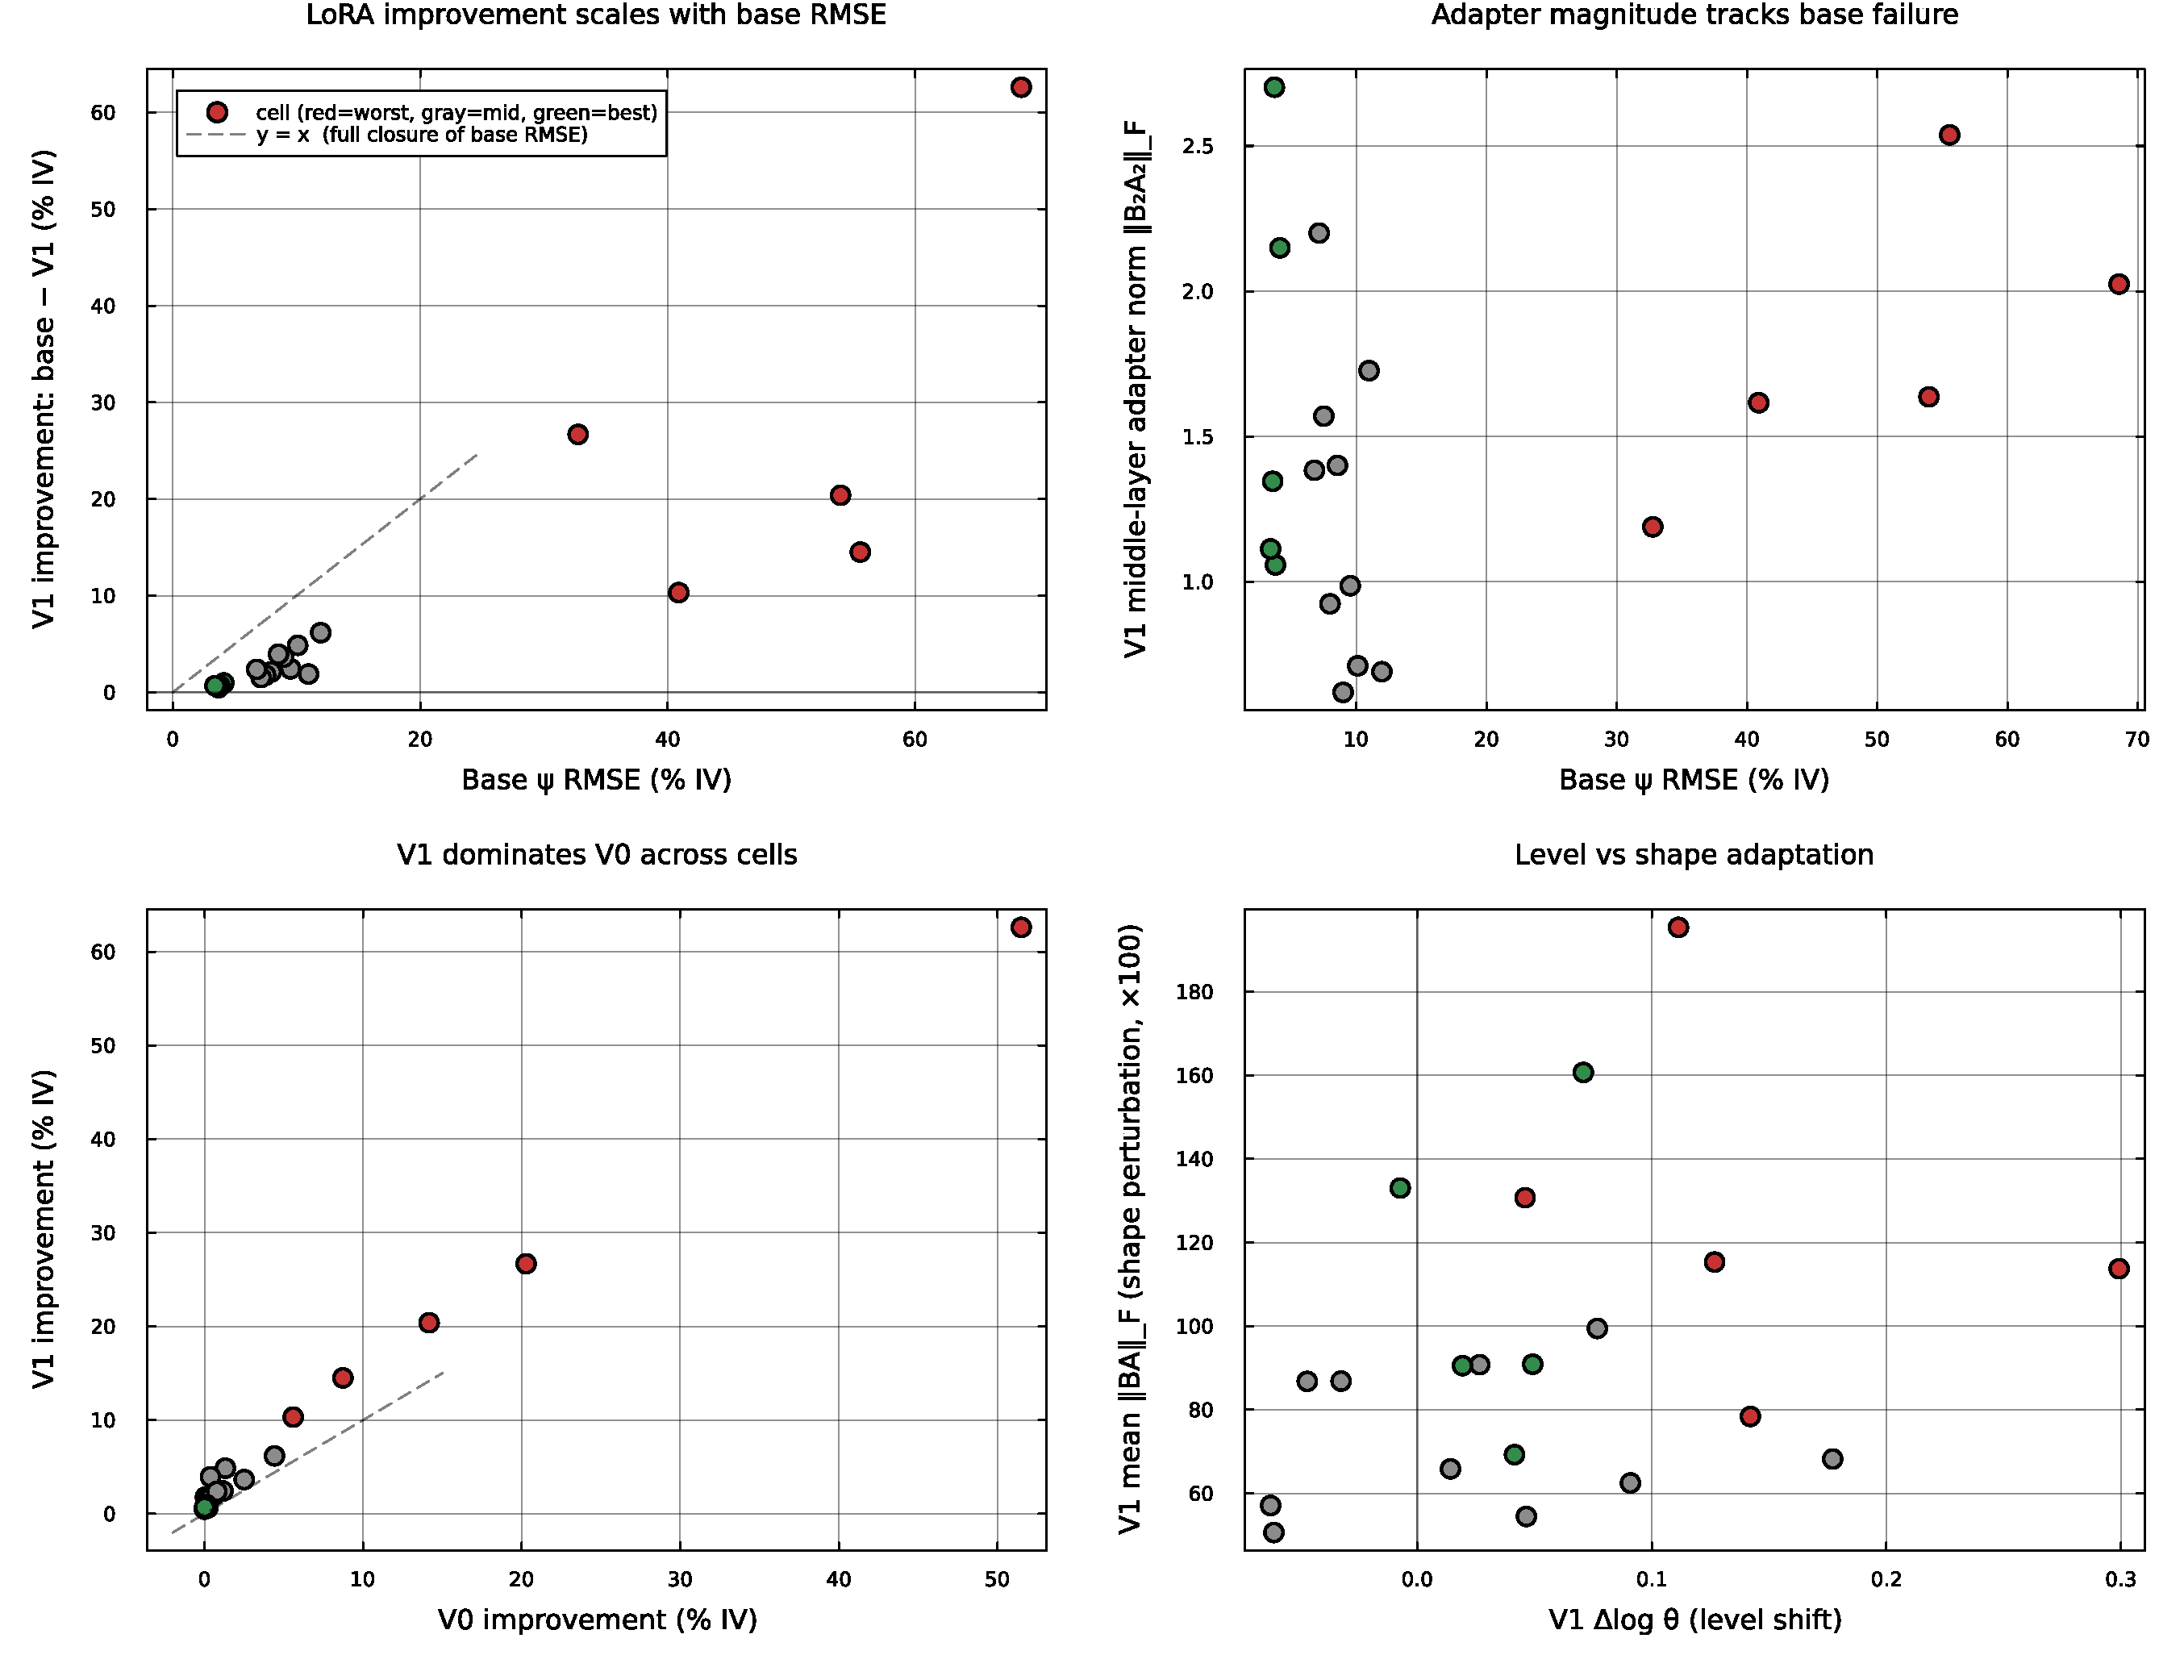
\includegraphics[width=\textwidth]{sections/figures/lora_sweep_summary.pdf}
\caption{LoRA sweep diagnostics across 20 (ticker, date) cells. (A) V1 improvement scales with base RMSE: red points are problem cells, gray middle, green controls. The diagonal marks full-closure (V1 RMSE = 0). (B) The middle-layer adapter norm $\|B_2 A_2\|_F$ tracks base RMSE, consistent with the LoRA-on-transformers pattern of intermediate-representation adaptation. (C) V1 dominates V0 across cells; the diagonal would mark equal improvement. (D) V1 partitions its budget between a small level shift ($\Delta\log\theta$ near zero on most cells) and a larger shape perturbation (mean $\|BA\|_F$), with the four shape-heavy outliers being the four highest-RMSE problem cells.}\label{fig:lora_sweep}
\end{figure}

\subsection{LLY 04-28 entry-edge case study}\label{sec:supp_lora_lly}

The LLY 04-28 cell appeared as a single row in Table~\ref{tab:lora_sweep} (sweep position: middle cell, base RMSE 15.66\%, V1 RMSE 4.34\% reported here in detail rather than the 04-22 row above), and we re-priced its $30\Delta$ put and call under each adapter variant to translate the slice-RMSE improvement into a dollar entry-edge story.

\begin{table}[ht]
\centering
\caption{LLY 04-28 entry-edge case study, the failure case that motivated the adapter. Market mids and $\psi_{\text{NN}}$-implied fair values are reported alongside V0 (level-only) and V1 (rank-2 LoRA + level). Variant 0 over-prices both $30\Delta$ contracts because the global level lift needed to fit the wings over-shoots the $30\Delta$ strikes; Variant 1's rank-2 shape perturbation lifts the wings while leaving the near-the-money region near market, closing the $-\$1.80$ call edge to $+\$0.46$ and the $-\$1.35$ put edge to $-\$1.15$.}\label{tab:lora_lly_edges}
\begin{tabular}{lrrrr|rrr}
\toprule
& Market mid & Base FV & V0 FV & V1 FV & Base edge & V0 edge & V1 edge \\
\midrule
LLY \$825 put  & \$23.30 & \$21.95 & \$29.45 & \$22.15 & $-\$1.35$ & $+\$6.15$ & $-\$1.15$ \\
LLY \$940 call & \$20.76 & \$18.96 & \$26.20 & \$21.22 & $-\$1.80$ & $+\$5.44$ & $+\$0.46$ \\
\midrule
Slice RMSE on 04-28 (\% IV) & --- & 15.66 & 11.78 & \textbf{4.34} & --- & --- & --- \\
\bottomrule
\end{tabular}
\end{table}

\subsection{No-arbitrage audit on V1-adapted surfaces}\label{sec:supp_lora_arb}

The rank-2 adapter carries no structural arbitrage constraint, so we re-evaluated the static-arbitrage diagnostic of §\ref{sec:supp_static_arb} on each of the 20 cells under the V1-adapted $\psi_{\text{NN}}$ and compared to the base. The aggregate butterfly violation rate rose from $9.78\%$ ($704 / 7{,}200$) to $12.74\%$ ($917 / 7{,}200$), and the calendar rate rose from $1.01\%$ ($77 / 7{,}600$) to $2.32\%$ ($176 / 7{,}600$). The amplification concentrated on the highest-base-RMSE cells where the adapter perturbation was largest in absolute terms (INTC 04-23, AMD 04-23, QCOM 04-23 each saw their butterfly rate triple), and six of the twenty cells actually saw violations decrease under adaptation. The unconstrained adapter is therefore not free: aggressive cells trade slice-RMSE accuracy for wing-arbitrage cleanliness. The natural extension --- a Variant 2 with an arbitrage-penalty term in the adapter loss --- is straightforward in the LoRA framework but was not implemented here.

\begin{figure}[ht]
\centering
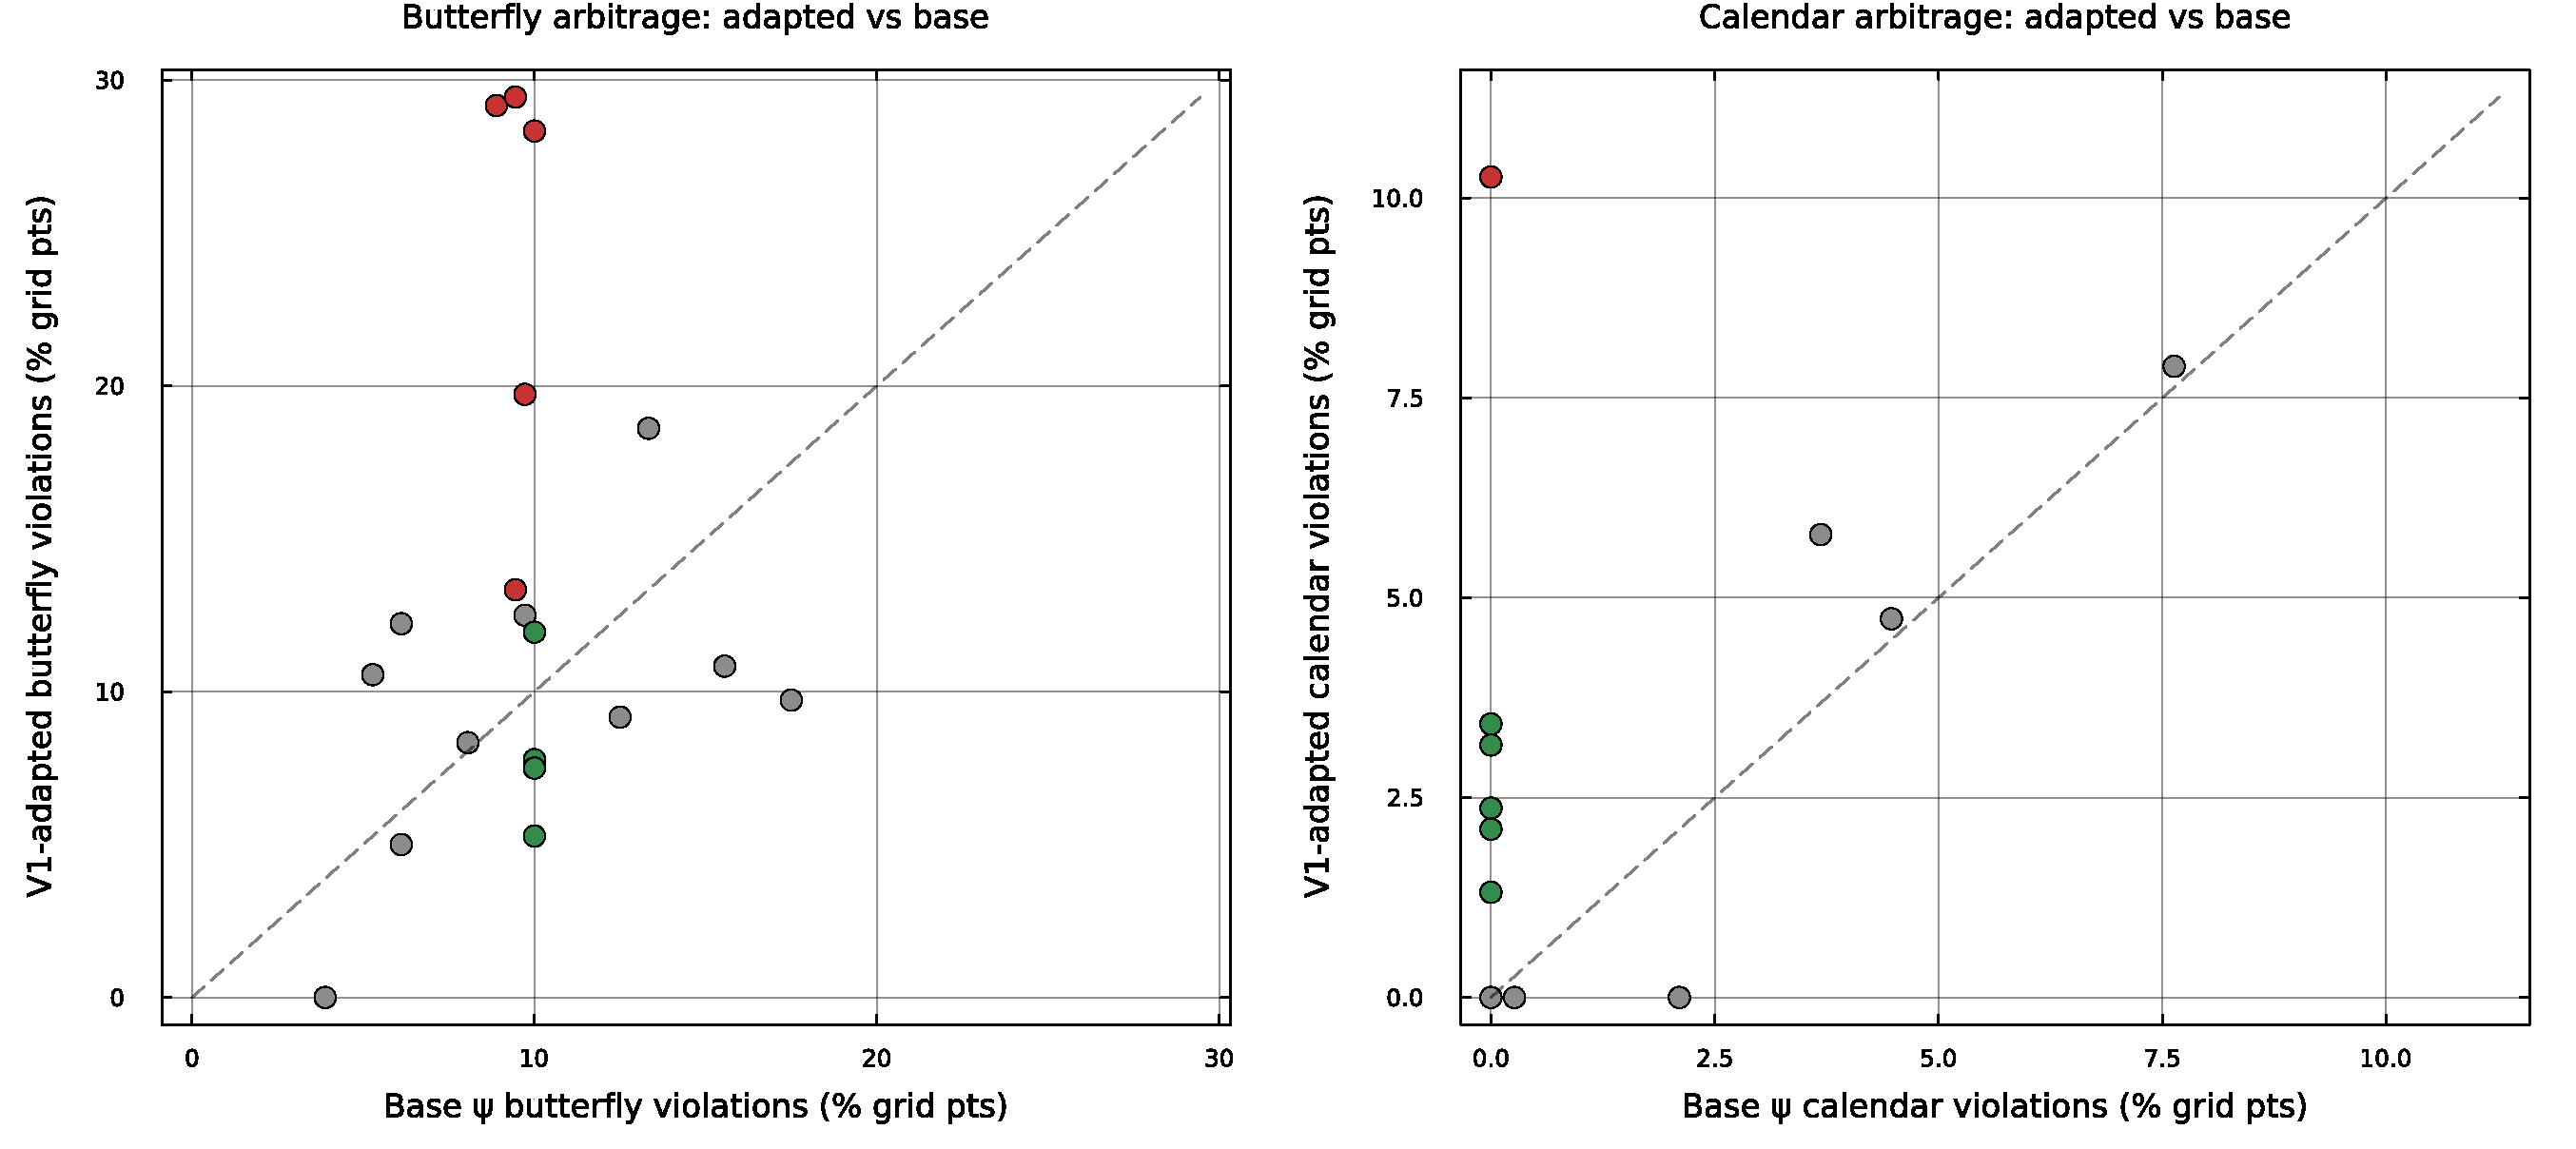
\includegraphics[width=\textwidth]{sections/figures/lora_arbitrage_audit.pdf}
\caption{No-arbitrage audit on V1-adapted surfaces. Left: butterfly violation rates (\% of $20 \times 20$ grid points where $\partial^2 C/\partial K^2 < 0$) for the V1-adapted surface versus the base, across the 20 sweep cells. Right: calendar violation rates (\% where $\partial C / \partial T < 0$). Red = problem cells, gray = middle, green = control. The dashed line is parity; points above amplify violations, points below reduce them. Six of twenty cells lie below parity; the rest sit slightly above, with three Tech-04-23 cells producing the largest amplification.}\label{fig:lora_arb_audit}
\end{figure}

\subsection{Streaming trigger ROC}\label{sec:supp_lora_trigger}

We evaluated the streaming trigger of §\ref{sec:lora_trigger} on every (ticker, date) cell in the $31 \times 15$ corpus ($457$ filtered cells after the $N_{\text{obs}} \geq 10$ filter). Ground truth was defined as the binary indicator $\text{RMSE}_t > 12\%$ IV ($112 / 457$ positive cells). The trigger was run with the absolute floor $\tau_{\text{abs}} = 10\%$ fixed and the relative threshold $\tau_z$ swept from $0$ to $6$. The trailing window length was $4$ non-flagged dates per ticker, with $1.4826 \times \mathrm{MAD}$ as the robust scale. Flagged dates were excluded from the trailing baseline for subsequent decisions on the same ticker.

\begin{table}[ht]
\centering
\caption{Streaming-trigger operating-point summary on the $31 \times 15$ corpus ($457$ cells, $112$ truth-positive). The Youden-optimal point ($\tau_z = 0$) recovers $74\%$ of refit-needed cells with $67\%$ precision; the more conservative $\tau_z = 1.5$ default trades precision for fewer false positives. The remaining false negatives concentrate on the four-date warm-up window where no streaming statistic can discriminate without trailing data.}\label{tab:lora_trigger_roc}
\begin{tabular}{lrrr}
\toprule
$\tau_z$ & TPR (recall) & FPR & Precision \\
\midrule
0.00 (Youden-optimal) & 0.741 & 0.119 & 0.669 \\
0.75 & 0.696 & 0.101 & 0.690 \\
1.50 (conservative default) & 0.670 & 0.096 & 0.694 \\
3.00 & 0.545 & 0.078 & 0.693 \\
6.00 & 0.312 & 0.035 & 0.745 \\
\bottomrule
\end{tabular}
\end{table}

\begin{figure}[ht]
\centering
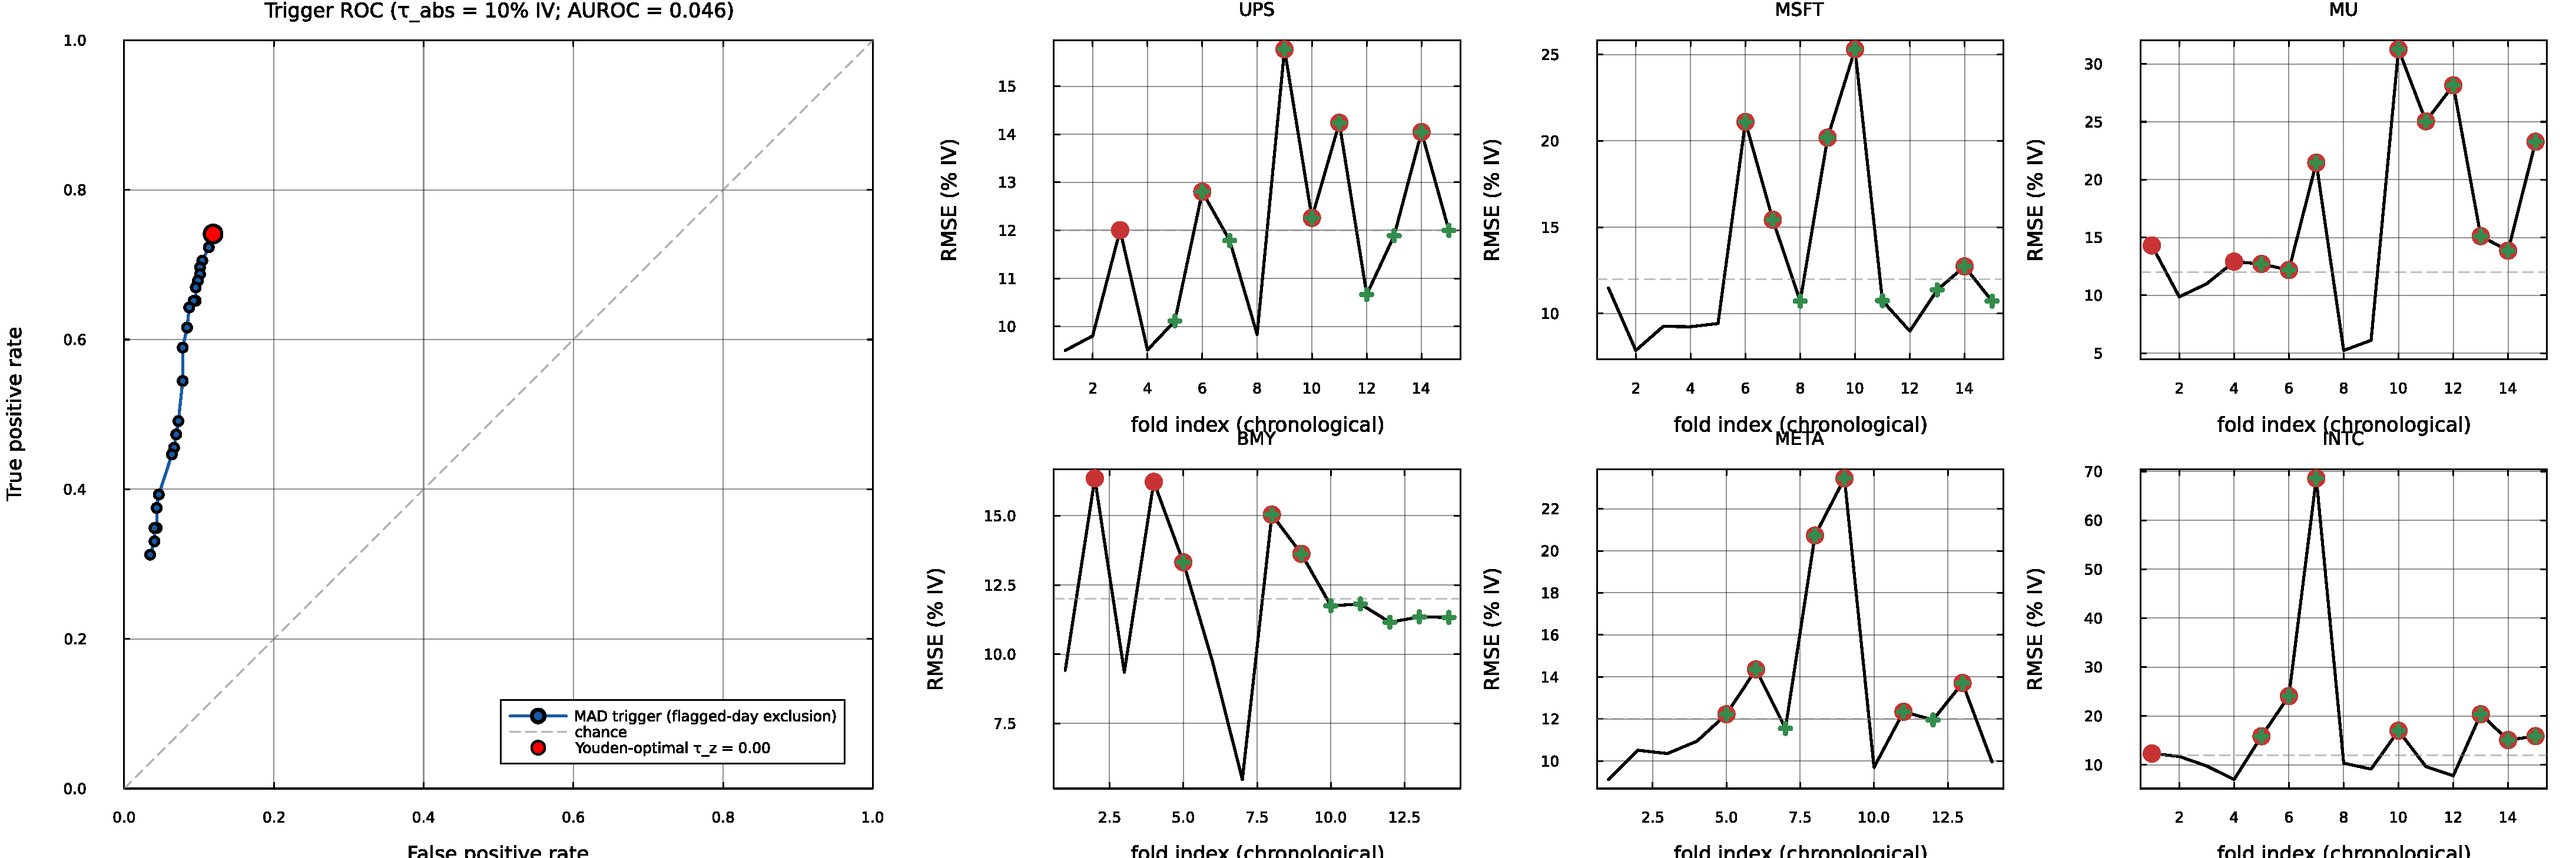
\includegraphics[width=\textwidth]{sections/figures/lora_trigger_roc.pdf}
\caption{Streaming refit trigger. Left: ROC curve obtained by sweeping $\tau_z$ at fixed $\tau_{\text{abs}} = 10\%$ IV; the Youden-optimal operating point is marked red, and the curve is bounded away from $\mathrm{TPR} = 1$ by the four-date warm-up window (which contains $\sim 27\%$ of truth-positive cells, none of which can be flagged without trailing data). Right: per-ticker chronological RMSE timelines for the six most-flagged tickers, with red filled circles marking truth-positive cells (base RMSE above the 12\% refit-needed threshold) and green crosses marking the trigger's flag decisions at the conservative $\tau_z = 1.5$ default. The INTC trace shows the four-date sequence ($\text{04-21}, \text{04-22}, \text{04-23}, \text{04-28}$) that the contamination-fix-equipped trigger correctly captures across the earnings-print event and the subsequent regime echo.}\label{fig:lora_trigger}
\end{figure}
